% Options for packages loaded elsewhere
\PassOptionsToPackage{unicode}{hyperref}
\PassOptionsToPackage{hyphens}{url}
\PassOptionsToPackage{dvipsnames,svgnames,x11names}{xcolor}
%
\documentclass[
  letterpaper,
  DIV=11,
  numbers=noendperiod]{scrartcl}

\usepackage{amsmath,amssymb}
\usepackage{iftex}
\ifPDFTeX
  \usepackage[T1]{fontenc}
  \usepackage[utf8]{inputenc}
  \usepackage{textcomp} % provide euro and other symbols
\else % if luatex or xetex
  \usepackage{unicode-math}
  \defaultfontfeatures{Scale=MatchLowercase}
  \defaultfontfeatures[\rmfamily]{Ligatures=TeX,Scale=1}
\fi
\usepackage{lmodern}
\ifPDFTeX\else  
    % xetex/luatex font selection
\fi
% Use upquote if available, for straight quotes in verbatim environments
\IfFileExists{upquote.sty}{\usepackage{upquote}}{}
\IfFileExists{microtype.sty}{% use microtype if available
  \usepackage[]{microtype}
  \UseMicrotypeSet[protrusion]{basicmath} % disable protrusion for tt fonts
}{}
\makeatletter
\@ifundefined{KOMAClassName}{% if non-KOMA class
  \IfFileExists{parskip.sty}{%
    \usepackage{parskip}
  }{% else
    \setlength{\parindent}{0pt}
    \setlength{\parskip}{6pt plus 2pt minus 1pt}}
}{% if KOMA class
  \KOMAoptions{parskip=half}}
\makeatother
\usepackage{xcolor}
\usepackage[left=1in,right=1in,top=1in,bottom=1in]{geometry}
\setlength{\emergencystretch}{3em} % prevent overfull lines
\setcounter{secnumdepth}{-\maxdimen} % remove section numbering
% Make \paragraph and \subparagraph free-standing
\makeatletter
\ifx\paragraph\undefined\else
  \let\oldparagraph\paragraph
  \renewcommand{\paragraph}{
    \@ifstar
      \xxxParagraphStar
      \xxxParagraphNoStar
  }
  \newcommand{\xxxParagraphStar}[1]{\oldparagraph*{#1}\mbox{}}
  \newcommand{\xxxParagraphNoStar}[1]{\oldparagraph{#1}\mbox{}}
\fi
\ifx\subparagraph\undefined\else
  \let\oldsubparagraph\subparagraph
  \renewcommand{\subparagraph}{
    \@ifstar
      \xxxSubParagraphStar
      \xxxSubParagraphNoStar
  }
  \newcommand{\xxxSubParagraphStar}[1]{\oldsubparagraph*{#1}\mbox{}}
  \newcommand{\xxxSubParagraphNoStar}[1]{\oldsubparagraph{#1}\mbox{}}
\fi
\makeatother

\usepackage{color}
\usepackage{fancyvrb}
\newcommand{\VerbBar}{|}
\newcommand{\VERB}{\Verb[commandchars=\\\{\}]}
\DefineVerbatimEnvironment{Highlighting}{Verbatim}{commandchars=\\\{\}}
% Add ',fontsize=\small' for more characters per line
\usepackage{framed}
\definecolor{shadecolor}{RGB}{241,243,245}
\newenvironment{Shaded}{\begin{snugshade}}{\end{snugshade}}
\newcommand{\AlertTok}[1]{\textcolor[rgb]{0.68,0.00,0.00}{#1}}
\newcommand{\AnnotationTok}[1]{\textcolor[rgb]{0.37,0.37,0.37}{#1}}
\newcommand{\AttributeTok}[1]{\textcolor[rgb]{0.40,0.45,0.13}{#1}}
\newcommand{\BaseNTok}[1]{\textcolor[rgb]{0.68,0.00,0.00}{#1}}
\newcommand{\BuiltInTok}[1]{\textcolor[rgb]{0.00,0.23,0.31}{#1}}
\newcommand{\CharTok}[1]{\textcolor[rgb]{0.13,0.47,0.30}{#1}}
\newcommand{\CommentTok}[1]{\textcolor[rgb]{0.37,0.37,0.37}{#1}}
\newcommand{\CommentVarTok}[1]{\textcolor[rgb]{0.37,0.37,0.37}{\textit{#1}}}
\newcommand{\ConstantTok}[1]{\textcolor[rgb]{0.56,0.35,0.01}{#1}}
\newcommand{\ControlFlowTok}[1]{\textcolor[rgb]{0.00,0.23,0.31}{\textbf{#1}}}
\newcommand{\DataTypeTok}[1]{\textcolor[rgb]{0.68,0.00,0.00}{#1}}
\newcommand{\DecValTok}[1]{\textcolor[rgb]{0.68,0.00,0.00}{#1}}
\newcommand{\DocumentationTok}[1]{\textcolor[rgb]{0.37,0.37,0.37}{\textit{#1}}}
\newcommand{\ErrorTok}[1]{\textcolor[rgb]{0.68,0.00,0.00}{#1}}
\newcommand{\ExtensionTok}[1]{\textcolor[rgb]{0.00,0.23,0.31}{#1}}
\newcommand{\FloatTok}[1]{\textcolor[rgb]{0.68,0.00,0.00}{#1}}
\newcommand{\FunctionTok}[1]{\textcolor[rgb]{0.28,0.35,0.67}{#1}}
\newcommand{\ImportTok}[1]{\textcolor[rgb]{0.00,0.46,0.62}{#1}}
\newcommand{\InformationTok}[1]{\textcolor[rgb]{0.37,0.37,0.37}{#1}}
\newcommand{\KeywordTok}[1]{\textcolor[rgb]{0.00,0.23,0.31}{\textbf{#1}}}
\newcommand{\NormalTok}[1]{\textcolor[rgb]{0.00,0.23,0.31}{#1}}
\newcommand{\OperatorTok}[1]{\textcolor[rgb]{0.37,0.37,0.37}{#1}}
\newcommand{\OtherTok}[1]{\textcolor[rgb]{0.00,0.23,0.31}{#1}}
\newcommand{\PreprocessorTok}[1]{\textcolor[rgb]{0.68,0.00,0.00}{#1}}
\newcommand{\RegionMarkerTok}[1]{\textcolor[rgb]{0.00,0.23,0.31}{#1}}
\newcommand{\SpecialCharTok}[1]{\textcolor[rgb]{0.37,0.37,0.37}{#1}}
\newcommand{\SpecialStringTok}[1]{\textcolor[rgb]{0.13,0.47,0.30}{#1}}
\newcommand{\StringTok}[1]{\textcolor[rgb]{0.13,0.47,0.30}{#1}}
\newcommand{\VariableTok}[1]{\textcolor[rgb]{0.07,0.07,0.07}{#1}}
\newcommand{\VerbatimStringTok}[1]{\textcolor[rgb]{0.13,0.47,0.30}{#1}}
\newcommand{\WarningTok}[1]{\textcolor[rgb]{0.37,0.37,0.37}{\textit{#1}}}

\providecommand{\tightlist}{%
  \setlength{\itemsep}{0pt}\setlength{\parskip}{0pt}}\usepackage{longtable,booktabs,array}
\usepackage{calc} % for calculating minipage widths
% Correct order of tables after \paragraph or \subparagraph
\usepackage{etoolbox}
\makeatletter
\patchcmd\longtable{\par}{\if@noskipsec\mbox{}\fi\par}{}{}
\makeatother
% Allow footnotes in longtable head/foot
\IfFileExists{footnotehyper.sty}{\usepackage{footnotehyper}}{\usepackage{footnote}}
\makesavenoteenv{longtable}
\usepackage{graphicx}
\makeatletter
\def\maxwidth{\ifdim\Gin@nat@width>\linewidth\linewidth\else\Gin@nat@width\fi}
\def\maxheight{\ifdim\Gin@nat@height>\textheight\textheight\else\Gin@nat@height\fi}
\makeatother
% Scale images if necessary, so that they will not overflow the page
% margins by default, and it is still possible to overwrite the defaults
% using explicit options in \includegraphics[width, height, ...]{}
\setkeys{Gin}{width=\maxwidth,height=\maxheight,keepaspectratio}
% Set default figure placement to htbp
\makeatletter
\def\fps@figure{htbp}
\makeatother

\usepackage{booktabs}
\usepackage{longtable}
\usepackage{array}
\usepackage{multirow}
\usepackage{wrapfig}
\usepackage{float}
\usepackage{colortbl}
\usepackage{pdflscape}
\usepackage{tabu}
\usepackage{threeparttable}
\usepackage{threeparttablex}
\usepackage[normalem]{ulem}
\usepackage{makecell}
\usepackage{xcolor}
\usepackage{fvextra}
\DefineVerbatimEnvironment{Highlighting}{Verbatim}{breaklines,commandchars=\\\{\}}
\DefineVerbatimEnvironment{OutputCode}{Verbatim}{breaklines,commandchars=\\\{\}}
\KOMAoption{captions}{tableheading}
\makeatletter
\@ifpackageloaded{caption}{}{\usepackage{caption}}
\AtBeginDocument{%
\ifdefined\contentsname
  \renewcommand*\contentsname{Table of contents}
\else
  \newcommand\contentsname{Table of contents}
\fi
\ifdefined\listfigurename
  \renewcommand*\listfigurename{List of Figures}
\else
  \newcommand\listfigurename{List of Figures}
\fi
\ifdefined\listtablename
  \renewcommand*\listtablename{List of Tables}
\else
  \newcommand\listtablename{List of Tables}
\fi
\ifdefined\figurename
  \renewcommand*\figurename{Figure}
\else
  \newcommand\figurename{Figure}
\fi
\ifdefined\tablename
  \renewcommand*\tablename{Table}
\else
  \newcommand\tablename{Table}
\fi
}
\@ifpackageloaded{float}{}{\usepackage{float}}
\floatstyle{ruled}
\@ifundefined{c@chapter}{\newfloat{codelisting}{h}{lop}}{\newfloat{codelisting}{h}{lop}[chapter]}
\floatname{codelisting}{Listing}
\newcommand*\listoflistings{\listof{codelisting}{List of Listings}}
\makeatother
\makeatletter
\makeatother
\makeatletter
\@ifpackageloaded{caption}{}{\usepackage{caption}}
\@ifpackageloaded{subcaption}{}{\usepackage{subcaption}}
\makeatother

\ifLuaTeX
  \usepackage{selnolig}  % disable illegal ligatures
\fi
\usepackage{bookmark}

\IfFileExists{xurl.sty}{\usepackage{xurl}}{} % add URL line breaks if available
\urlstyle{same} % disable monospaced font for URLs
\hypersetup{
  pdftitle={Case Study 1: A Statistical Analysis of the Anomaly in the U.S. 2000 Presidential Election},
  pdfauthor={Miya Dang, Mia Tran},
  colorlinks=true,
  linkcolor={blue},
  filecolor={Maroon},
  citecolor={Blue},
  urlcolor={Blue},
  pdfcreator={LaTeX via pandoc}}


\title{Case Study 1: A Statistical Analysis of the Anomaly in the U.S.
2000 Presidential Election}
\author{Miya Dang, Mia Tran}
\date{2025-03-05}

\begin{document}
\maketitle


\subsubsection{Introduction}\label{introduction}

The U.S. presidential election in 2000 between George W. Bush and Al
Gore was one of the closest in history, with its final outcome dependent
on the results in the state of Florida. Ultimately, Bush secured victory
by a margin of fewer than 400 votes. However, Democratic voters in Palm
Beach County argued that a confusing ``butterfly'' ballot layout led
them to mistakenly vote for Reform Party candidate Pat Buchanan instead
of Gore. This claim was supported by evidence showing that Buchanan
received an unusually high percentage of votes in the county, along with
a significant number of discarded ballots where voters had marked two
choices.

In this case study, we will model the relationship between Bush and
Buchanan votes in 2000 across Florida (excluding Palm Beach County to
assess its anomaly) to answer two questions:

\begin{itemize}
\tightlist
\item
  \emph{Was the number of votes for Buchanan in Palm Beach County
  statistically unusual compared to other Florida counties?}
\item
  \emph{What is the estimated number of votes intended for Gore but cast
  for Buchanan in Palm Beach County?}
\end{itemize}

\subsubsection{Data Description}\label{data-description}

The dataset contains the vote counts for Buchanan and Bush in 2000
across all 67 counties in Florida.

\textbf{Summary Statistics:}

\begin{verbatim}
    Bush2000       Buchanan2000   
 Min.   :  1316   Min.   :   9.0  
 1st Qu.:  4746   1st Qu.:  46.5  
 Median : 20196   Median : 114.0  
 Mean   : 43356   Mean   : 258.5  
 3rd Qu.: 56542   3rd Qu.: 285.5  
 Max.   :289456   Max.   :3407.0  
\end{verbatim}

\begin{itemize}
\item
  Summary statistics indicate that, overall, Bush received significantly
  higher votes than Buchanan.
\item
  Both variables have means much higher than their medians, indicating a
  strong right skew. This suggests that most counties had relatively low
  vote counts, while a small number had exceptionally high vote counts.
\item
  The maximum number of Buchanan votes was 3,407, far exceeding the
  third quantile of 285.5. This vote count came from Palm Beach County,
  suggesting that it is an outlier.
\end{itemize}

\textbf{Accompanying Graph:}

The scatterplot below visualizes the relationship between Bush votes
(x-axis) and Buchanan votes (y-axis) for all 67 counties:

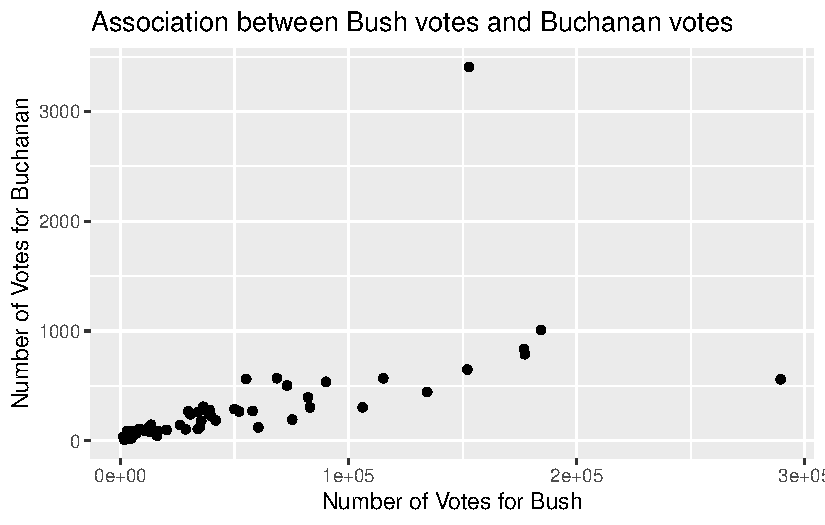
\includegraphics{SDS-291-case-study-1_files/figure-pdf/unnamed-chunk-3-1.pdf}

There is a general positive trend, as counties with more Bush votes also
tended to have more Buchanan votes. Palm Beach County (the mark on the
top of the graph) is a notable outlier with unexpectedly high Buchanan
votes (3,407). This graph shows that the data is highly left-skewed,
raising concerns about potential violations of model assumptions, which
we will examine in the next section.

\subsubsection{Modeling Process and
Results}\label{modeling-process-and-results}

Originally, we fitted a simple linear regression model for predicting
Buchanan votes from Bush votes. Let \(Buchanan\) denote the votes for
Buchanan in Palm Beach County and \(Bush\) denote the votes for Bush in
Palm Beach County. Our original model is in the form:
\[Buchanan = \beta_0 + \beta_1\left(Bush\right).\] where:

\begin{itemize}
\tightlist
\item
  \(\beta_0\) is the intercept of the model, representing the expected
  value of the number of votes for Buchanan when the number of votes for
  Bush is 0.
\end{itemize}

\begin{itemize}
\tightlist
\item
  \(\beta_1\) represents the percentage change in Buchanan's votes for a
  1\% increase in Bush's votes. The table below shows the summary
  statistics of the simple linear regression model:
\end{itemize}

\begin{table}[H]
\centering
\begin{tabular}[t]{lcccc}
\toprule
  & Estimate & Std. Error & t value & Pr(>|t|)\\
\midrule
(Intercept) & 65.5735 & 17.3304 & 3.7837 & 0.00034\\
Bush2000 & 0.0035 & 0.0003 & 13.9226 & 0.00000\\
\bottomrule
\end{tabular}
\end{table}

We proceeded to check the conditions for t-based inference with the
simple linear regression model above. According to the data context, the
Independence assumption is likely satisfied since the data consists of
separate observations for each county in Florida (excluding Palm Beach
County). Since each county reports its election results independently,
the votes counted in one county do not directly influence the votes in
another. Additionally, while counties may share some similarities, they
operate as distinct political and administrative entities, each with its
own local voting trends, demographics, and electoral processes, reducing
the likelihood of systematic dependence between counties. The residual
vs.~fitted value plot below allows us to check the Linearity and Equal
Variance conditions:

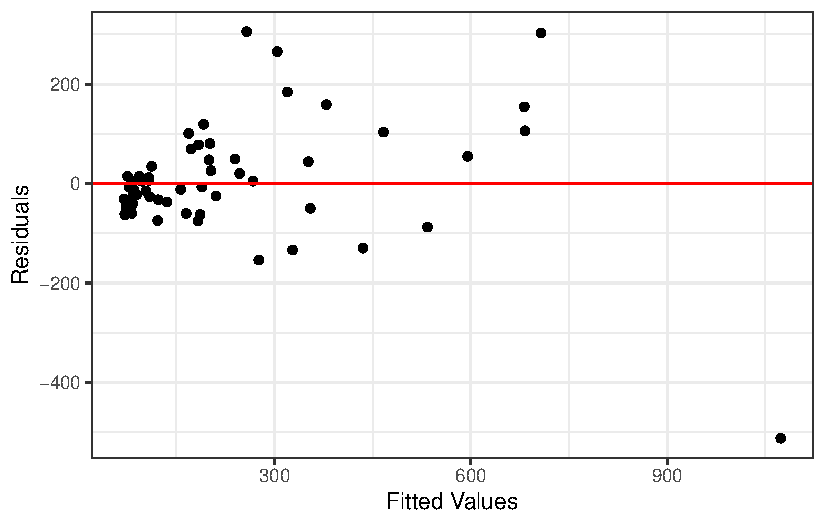
\includegraphics{SDS-291-case-study-1_files/figure-pdf/unnamed-chunk-5-1.pdf}

The residuals vs.~fitted values plot indicates that both the Linearity
and Equal Variance assumptions are violated. The clustering of residuals
at the start of the line suggests a non-random pattern, violating the
Linearity assumption. Additionally, the inconsistent vertical spread
across fitted values indicates a lack of constant variance, suggesting a
violation of the Equal Variance assumption.

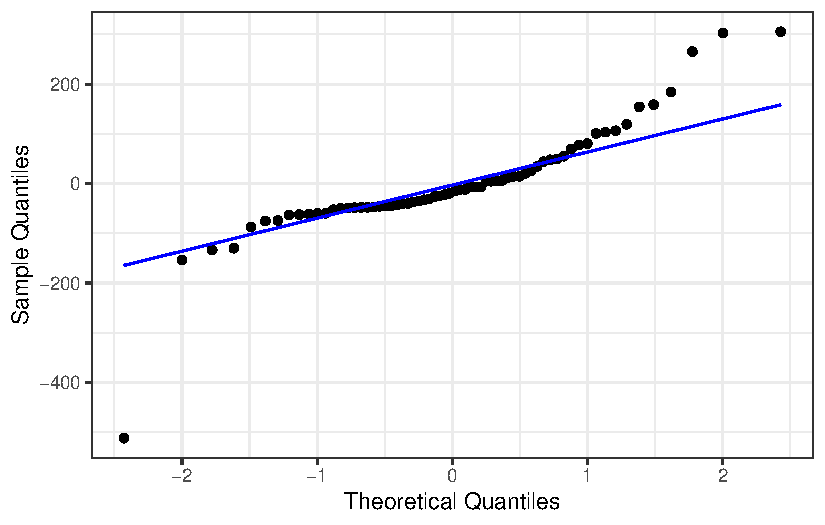
\includegraphics{SDS-291-case-study-1_files/figure-pdf/unnamed-chunk-6-1.pdf}

The Q-Q plot suggests a violation of the Normality assumption, as the
residuals deviate from the reference line not only at the extremes but
also in the middle, indicating that they do not follow a normal
distribution.

Since the Linearity, Equal Variance, and Normality assumptions are
violated, our simple linear regression model is not appropriate for
modeling the relationship between Buchanan's votes and Bush's votes. To
address this, we applied a logarithmic transformation to the model.

Let \(log(Buchanan)\) denote the natural logarithm of the votes for
Buchanan in Palm Beach County and \(log(Bush)\) denote the natural
logarithm the votes for Bush in Palm Beach County. Our transformed
linear regression model is:
\[E[log(Buchanan) | log(Bush)] = \beta_0 + \beta_1log(Bush).\]where:

\begin{itemize}
\item
  \(\beta_0\) is the intercept of the model, representing the expected
  value of \(log(Buchanan)\) when \(log(Bush) = 0\). Since
  \(log(1) = 0\), this means \(\beta_0\) represents the expected value
  of \(log(Buchanan)\) when the numbers of votes for Bush is 1.
\item
  \(\beta_1\) represents the elasticity of Buchanan's votes with respect
  to Bush's votes. A 1\% increase in Bush's votes is associated with a
  \(\beta_1\)\% change in Buchanan's votes.
\end{itemize}

The table below shows the summary statistics of the transformed linear
regression model:

\begin{table}[H]
\centering
\begin{tabular}[t]{lcccc}
\toprule
  & Estimate & Std. Error & t value & Pr(>|t|)\\
\midrule
(Intercept) & -2.3415 & 0.3544 & -6.6066 & 0\\
log(Bush2000) & 0.7310 & 0.0360 & 20.3229 & 0\\
\bottomrule
\end{tabular}
\end{table}

From the table, our transformed linear regression model can be written
as: \[E[log(Buchanan) | log(Bush)] = -2.34 + 0.73log(Bush).\] The
standard error for the intercept and the slope is 0.354 and 0.036
respectively according to the table.

We proceeded to check the conditions for t-based inference with the
transformed regression model above. The residual vs.~fitted value plot
below allows us to check the Linearity and Equal Variance conditions:

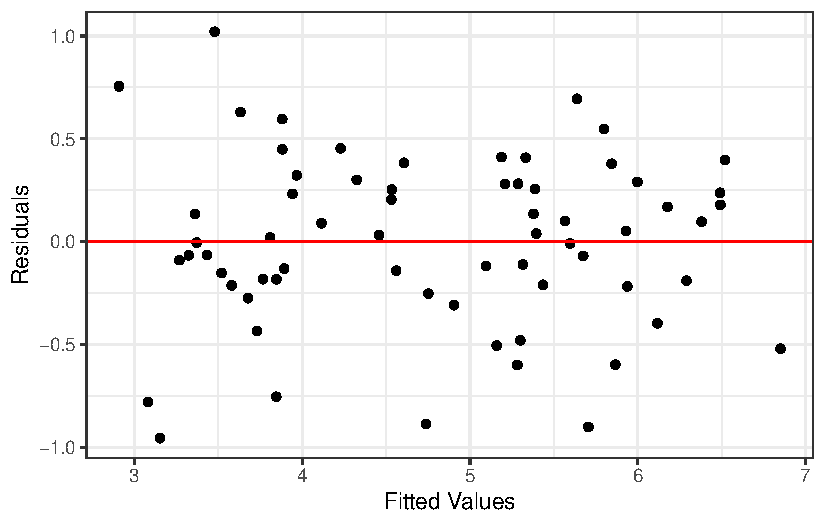
\includegraphics{SDS-291-case-study-1_files/figure-pdf/unnamed-chunk-8-1.pdf}

The residuals vs.~fitted values plot indicates that both the Linearity
and Equal Variance assumptions are now satisfied. The residuals scatter
in random pattern around the \(y = 0\), satisfying the Linearity
assumption. Additionally, the fitted values follow a more consistent
vertical spread, indicating constant variance and satisfying the Equal
Variance assumption.

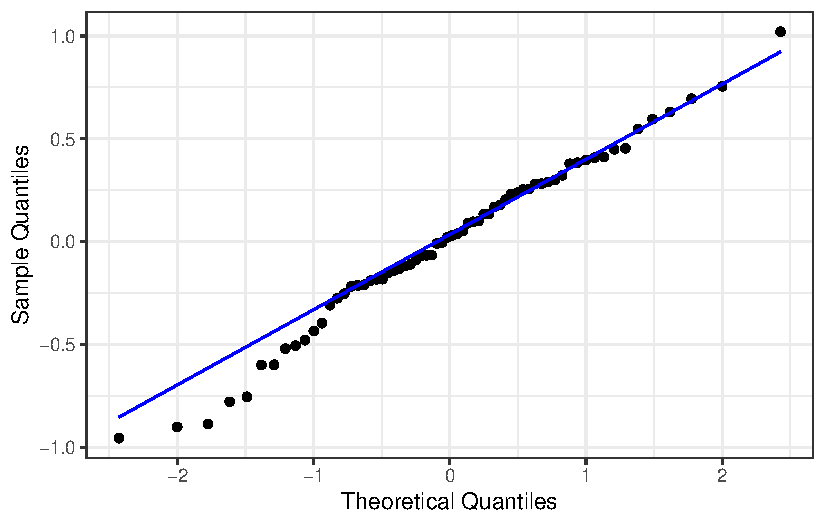
\includegraphics{SDS-291-case-study-1_files/figure-pdf/unnamed-chunk-9-1.pdf}

The Q-Q plot suggests a significant improvement in the normality
assumption. While the residuals slightly deviate from the reference line
at the beginning, they align more closely in the middle, indicating that
they approximately follow a normal distribution.

We obtained a 95\% prediction interval for the number of predicted
Buchanan votes in Palm Beach County using this transformed fitted model:

\begin{table}[H]
\centering
\begin{tabular}[t]{ccc}
\toprule
Fitted & Lower & Upper\\
\midrule
592 & 251 & 1399\\
\bottomrule
\end{tabular}
\end{table}

The table above shows that the prediction interval is \([251, 1399]\).
We are 95\% confident that the votes for Buchanan when there are 152,846
votes for Bush (which is the number of votes for Bush in Palm Beach
County) will fall between 251 votes and 1,399 votes.

Buchanan's real vote from Palm Beach County in 2000 election is 3,407
votes. Compared to the prediction interval above, we can calculate that
an estimate for the likely number of votes intended for Gore but cast
for Buchanan in Palm Beach County falls between \([2008, 3156]\).

\subsubsection{Summary and Conclusions}\label{summary-and-conclusions}

\textbf{Key Findings}

\begin{itemize}
\item
  The Buchanan vote count in Palm Beach County during the 2000 election
  was statistically unusual.
\item
  An estimated 2,008 to 3,156 votes intended for Gore were likely
  miscast for Buchanan.
\item
  These results suggest that the ballot design may have altered the
  election outcome. Given that Gore lost Florida by fewer than 400
  votes, the potential miscast votes in Palm Beach County alone far
  exceed this margin.
\end{itemize}

\textbf{Limitations}

\begin{itemize}
\item
  The log-log transformation assumes a multiplicative relationship
  between Bush and Buchanan votes. While this transformation improved
  linearity, residual diagnostics revealed mild heteroscedasticity and a
  slightly left-skewed residual distribution. These imply that the
  prediction interval may underestimate uncertainty, particularly for
  counties with high Bush vote count like Palm Beach.
\item
  The model assumes that voter behavior is similar across all counties.
  However, many other factors could contribute to regional differences
  between voter behavior, such as candidate campaigns or other
  demographic factors.
\item
  The analysis demonstrate association and not causation. Further
  investigation would be necessary to definitively prove that the
  butterfly ballot caused the excess Buchanan votes.
\end{itemize}

\subsection{R Appendix}\label{r-appendix}

\begin{Shaded}
\begin{Highlighting}[]
\CommentTok{\# Loading necessary packages}
\FunctionTok{library}\NormalTok{(tidyverse)}
\FunctionTok{library}\NormalTok{(Sleuth2)}
\FunctionTok{library}\NormalTok{(broom)        }
\FunctionTok{library}\NormalTok{(kableExtra)   }

\CommentTok{\# Loading the data for case study one}
\NormalTok{election }\OtherTok{\textless{}{-}}\NormalTok{ Sleuth2}\SpecialCharTok{::}\NormalTok{ex0825}

\CommentTok{\# Summary statistics}
\FunctionTok{summary}\NormalTok{(election }\SpecialCharTok{\%\textgreater{}\%} \FunctionTok{select}\NormalTok{(Bush2000, Buchanan2000))}

\CommentTok{\# Creating a scatterplot for the relationship between Bush and Buchanan votes}
\NormalTok{election }\SpecialCharTok{|\textgreater{}}
  \FunctionTok{ggplot}\NormalTok{(}\FunctionTok{aes}\NormalTok{(}\AttributeTok{x =}\NormalTok{ Bush2000,}
             \AttributeTok{y =}\NormalTok{ Buchanan2000)) }\SpecialCharTok{+}
  \FunctionTok{geom\_point}\NormalTok{() }\SpecialCharTok{+}
  \FunctionTok{ggtitle}\NormalTok{(}\StringTok{"Association between Bush votes and Buchanan votes"}\NormalTok{) }\SpecialCharTok{+}
  \FunctionTok{xlab}\NormalTok{(}\StringTok{"Number of Votes for Bush"}\NormalTok{) }\SpecialCharTok{+} \FunctionTok{ylab}\NormalTok{(}\StringTok{"Number of Votes for Buchanan"}\NormalTok{)}

\CommentTok{\# Creating a second dataset with Palm Beach County excluded}
\NormalTok{election\_wo\_pb }\OtherTok{\textless{}{-}}\NormalTok{ election }\SpecialCharTok{|\textgreater{}}
  \FunctionTok{filter}\NormalTok{(County }\SpecialCharTok{!=} \StringTok{"Palm Beach"}\NormalTok{)}

\CommentTok{\# Fitting the regression line for mean Buchanan votes }
\CommentTok{\# as a function of Bush votes}
\NormalTok{election\_lm }\OtherTok{\textless{}{-}} \FunctionTok{lm}\NormalTok{(Buchanan2000 }\SpecialCharTok{\textasciitilde{}}\NormalTok{ Bush2000, }\AttributeTok{data =}\NormalTok{ election\_wo\_pb)}


\CommentTok{\# Creating the table summarizing the estimated coefficients of the model }
\CommentTok{\# and their corresponding standard errors}
\NormalTok{election\_lm\_table }\OtherTok{\textless{}{-}} \FunctionTok{summary}\NormalTok{(election\_lm)}\SpecialCharTok{$}\NormalTok{coefficients}
\NormalTok{election\_lm\_table }\SpecialCharTok{|\textgreater{}} \FunctionTok{kbl}\NormalTok{(}\AttributeTok{col.names =} \FunctionTok{c}\NormalTok{(}\StringTok{"Estimate"}\NormalTok{, }\StringTok{"Std. Error"}\NormalTok{,}
                                       \StringTok{"t value"}\NormalTok{, }\StringTok{"Pr(\textgreater{}|t|)"}\NormalTok{), }
                         \AttributeTok{align =} \StringTok{"c"}\NormalTok{,}
                         \AttributeTok{booktabs =}\NormalTok{ T,}
                         \AttributeTok{linesep=}\StringTok{""}\NormalTok{,}
                         \AttributeTok{digits =} \FunctionTok{c}\NormalTok{(}\DecValTok{4}\NormalTok{, }\DecValTok{4}\NormalTok{, }\DecValTok{4}\NormalTok{, }\DecValTok{4}\NormalTok{)) }\SpecialCharTok{|\textgreater{}}
  \FunctionTok{kable\_classic}\NormalTok{(}\AttributeTok{full\_width =}\NormalTok{ F, }\AttributeTok{latex\_options =} \FunctionTok{c}\NormalTok{(}\StringTok{"HOLD\_position"}\NormalTok{))}

\CommentTok{\# Creating the residuals{-}fitted plot to check }
\CommentTok{\# Linearity and Equal Variance for the original election model}
\NormalTok{election\_lm }\SpecialCharTok{|\textgreater{}}
  \FunctionTok{augment}\NormalTok{() }\SpecialCharTok{|\textgreater{}}
  \FunctionTok{ggplot}\NormalTok{(}\FunctionTok{aes}\NormalTok{(}\AttributeTok{x =}\NormalTok{ .fitted, }\AttributeTok{y =}\NormalTok{ .resid)) }\SpecialCharTok{+}
  \FunctionTok{geom\_point}\NormalTok{() }\SpecialCharTok{+}
  \FunctionTok{geom\_hline}\NormalTok{(}\AttributeTok{yintercept =} \DecValTok{0}\NormalTok{, }\AttributeTok{col =} \StringTok{"red"}\NormalTok{) }\SpecialCharTok{+}
  \FunctionTok{xlab}\NormalTok{(}\StringTok{"Fitted Values"}\NormalTok{) }\SpecialCharTok{+}
  \FunctionTok{ylab}\NormalTok{(}\StringTok{"Residuals"}\NormalTok{) }\SpecialCharTok{+}
  \FunctionTok{theme\_bw}\NormalTok{()}

\CommentTok{\# Creating the Q{-}Q plot as check Normality for the original election model}
\NormalTok{election\_lm }\SpecialCharTok{|\textgreater{}}
  \FunctionTok{augment}\NormalTok{() }\SpecialCharTok{|\textgreater{}}
  \FunctionTok{ggplot}\NormalTok{(}\FunctionTok{aes}\NormalTok{(}\AttributeTok{sample =}\NormalTok{ .resid)) }\SpecialCharTok{+}
  \FunctionTok{geom\_qq}\NormalTok{() }\SpecialCharTok{+}
  \FunctionTok{geom\_qq\_line}\NormalTok{(}\AttributeTok{col =} \StringTok{"blue"}\NormalTok{) }\SpecialCharTok{+}
  \FunctionTok{xlab}\NormalTok{(}\StringTok{"Theoretical Quantiles"}\NormalTok{) }\SpecialCharTok{+}
  \FunctionTok{ylab}\NormalTok{(}\StringTok{"Sample Quantiles"}\NormalTok{) }\SpecialCharTok{+}
  \FunctionTok{theme\_bw}\NormalTok{()}

\CommentTok{\# Transformation}
\NormalTok{transformed\_election\_lm }\OtherTok{\textless{}{-}} \FunctionTok{lm}\NormalTok{(}\FunctionTok{log}\NormalTok{(Buchanan2000) }\SpecialCharTok{\textasciitilde{}} \FunctionTok{log}\NormalTok{(Bush2000), election\_wo\_pb)}

\CommentTok{\# Creating the table summarizing the estimated coefficients of the model }
\CommentTok{\# and their corresponding standard errors}
\NormalTok{transformed\_election\_lm\_table\_1 }\OtherTok{\textless{}{-}} \FunctionTok{summary}\NormalTok{(transformed\_election\_lm)}\SpecialCharTok{$}\NormalTok{coefficients}
\NormalTok{transformed\_election\_lm\_table\_1 }\SpecialCharTok{|\textgreater{}} \FunctionTok{kbl}\NormalTok{(}\AttributeTok{col.names =} \FunctionTok{c}\NormalTok{(}\StringTok{"Estimate"}\NormalTok{, }\StringTok{"Std. Error"}\NormalTok{,}
                                       \StringTok{"t value"}\NormalTok{, }\StringTok{"Pr(\textgreater{}|t|)"}\NormalTok{), }
                         \AttributeTok{align =} \StringTok{"c"}\NormalTok{,}
                         \AttributeTok{booktabs =}\NormalTok{ T,}
                         \AttributeTok{linesep=}\StringTok{""}\NormalTok{,}
                         \AttributeTok{digits =} \FunctionTok{c}\NormalTok{(}\DecValTok{4}\NormalTok{, }\DecValTok{4}\NormalTok{, }\DecValTok{4}\NormalTok{, }\DecValTok{4}\NormalTok{)) }\SpecialCharTok{|\textgreater{}}
  \FunctionTok{kable\_classic}\NormalTok{(}\AttributeTok{full\_width =}\NormalTok{ F, }\AttributeTok{latex\_options =} \FunctionTok{c}\NormalTok{(}\StringTok{"HOLD\_position"}\NormalTok{))}

\CommentTok{\# Creating the residuals{-}fitted plot to check }
\CommentTok{\# Linearity and Equal Variance for the transformed election model}
\NormalTok{transformed\_election\_lm }\SpecialCharTok{|\textgreater{}}
  \FunctionTok{augment}\NormalTok{() }\SpecialCharTok{|\textgreater{}}
  \FunctionTok{ggplot}\NormalTok{(}\FunctionTok{aes}\NormalTok{(}\AttributeTok{x =}\NormalTok{ .fitted, }\AttributeTok{y =}\NormalTok{ .resid)) }\SpecialCharTok{+}
  \FunctionTok{geom\_point}\NormalTok{() }\SpecialCharTok{+}
  \FunctionTok{geom\_hline}\NormalTok{(}\AttributeTok{yintercept =} \DecValTok{0}\NormalTok{, }\AttributeTok{col =} \StringTok{"red"}\NormalTok{) }\SpecialCharTok{+}
  \FunctionTok{xlab}\NormalTok{(}\StringTok{"Fitted Values"}\NormalTok{) }\SpecialCharTok{+}
  \FunctionTok{ylab}\NormalTok{(}\StringTok{"Residuals"}\NormalTok{) }\SpecialCharTok{+}
  \FunctionTok{theme\_bw}\NormalTok{()}

\CommentTok{\# Creating the Q{-}Q plot as check Normality for the transformed election model}
\NormalTok{transformed\_election\_lm }\SpecialCharTok{|\textgreater{}}
  \FunctionTok{augment}\NormalTok{() }\SpecialCharTok{|\textgreater{}}
  \FunctionTok{ggplot}\NormalTok{(}\FunctionTok{aes}\NormalTok{(}\AttributeTok{sample =}\NormalTok{ .resid)) }\SpecialCharTok{+}
  \FunctionTok{geom\_qq}\NormalTok{() }\SpecialCharTok{+}
  \FunctionTok{geom\_qq\_line}\NormalTok{(}\AttributeTok{col =} \StringTok{"blue"}\NormalTok{) }\SpecialCharTok{+}
  \FunctionTok{xlab}\NormalTok{(}\StringTok{"Theoretical Quantiles"}\NormalTok{) }\SpecialCharTok{+}
  \FunctionTok{ylab}\NormalTok{(}\StringTok{"Sample Quantiles"}\NormalTok{) }\SpecialCharTok{+}
  \FunctionTok{theme\_bw}\NormalTok{()}

\CommentTok{\# Filter the original dataset to only Palm Beach Country}
\CommentTok{\# to create prediction interval}
\NormalTok{election\_pb }\OtherTok{\textless{}{-}}\NormalTok{ election }\SpecialCharTok{|\textgreater{}} \FunctionTok{filter}\NormalTok{(County }\SpecialCharTok{==} \StringTok{"Palm Beach"}\NormalTok{)}

\CommentTok{\# Creating a 95\% prediction interval for the number of}
\CommentTok{\# predicted Buchanan votes in Palm Beach County}
\CommentTok{\# after knowing the votes for Bush from Palm Beach County}
\CommentTok{\# and transform back the interval}
\NormalTok{new\_election }\OtherTok{\textless{}{-}} \FunctionTok{data.frame}\NormalTok{(}\AttributeTok{Bush2000 =} \DecValTok{152846}\NormalTok{)}
\NormalTok{transformed\_election\_lm\_table\_2 }\OtherTok{\textless{}{-}}\NormalTok{ transformed\_election\_lm }\SpecialCharTok{|\textgreater{}}
  \FunctionTok{augment}\NormalTok{(}\AttributeTok{newdata =}\NormalTok{ new\_election,}
          \AttributeTok{interval =} \StringTok{"prediction"}\NormalTok{,}
          \AttributeTok{conf.level =} \FloatTok{0.95}\NormalTok{) }\SpecialCharTok{|\textgreater{}}
  \FunctionTok{select}\NormalTok{(}\FunctionTok{c}\NormalTok{(}\StringTok{".fitted"}\NormalTok{, }\StringTok{".lower"}\NormalTok{, }\StringTok{".upper"}\NormalTok{)) }\SpecialCharTok{|\textgreater{}} \FunctionTok{exp}\NormalTok{()}

\CommentTok{\# Creating the table summarizing the converted prediction interval}
\CommentTok{\# of the transformed model}
\NormalTok{transformed\_election\_lm\_table\_2 }\SpecialCharTok{|\textgreater{}} \FunctionTok{kbl}\NormalTok{(}\AttributeTok{col.names =} \FunctionTok{c}\NormalTok{(}\StringTok{"Fitted"}\NormalTok{, }\StringTok{"Lower"}\NormalTok{,}
                                       \StringTok{"Upper"}\NormalTok{), }
                         \AttributeTok{align =} \StringTok{"c"}\NormalTok{,}
                         \AttributeTok{booktabs =}\NormalTok{ T,}
                         \AttributeTok{linesep=}\StringTok{""}\NormalTok{,}
                         \AttributeTok{digits =} \FunctionTok{c}\NormalTok{(}\DecValTok{0}\NormalTok{, }\DecValTok{0}\NormalTok{, }\DecValTok{0}\NormalTok{)) }\SpecialCharTok{|\textgreater{}}
  \FunctionTok{kable\_classic}\NormalTok{(}\AttributeTok{full\_width =}\NormalTok{ F, }\AttributeTok{latex\_options =} \FunctionTok{c}\NormalTok{(}\StringTok{"HOLD\_position"}\NormalTok{))}
\end{Highlighting}
\end{Shaded}





\end{document}
